\documentclass[a4paper]{article}

\usepackage[utf8]{inputenc}
\usepackage[spanish]{babel}
\usepackage[T1]{fontenc}
\usepackage{lmodern}
\usepackage{graphicx}
\usepackage{lastpage}
\usepackage{listings}
\usepackage{fancyhdr}
\usepackage{url}
\usepackage{color}
\usepackage{fullpage}
\usepackage{float}

\definecolor{lightgray}{rgb}{0.95,0.95,0.95}

\lstloadlanguages{Haskell}

\graphicspath{ {images/} }

\setlength{\footskip }{20pt}
\setlength{\headsep }{30pt}
\addtolength{\textheight}{-40pt}


\lstset{
  frame=none,
  xleftmargin=25pt,
  stepnumber=1,
  numbers=left,
  numbersep=5pt,
  numberstyle=\ttfamily\tiny\color[gray]{0.3},
  belowcaptionskip=\bigskipamount,
  captionpos=b,
  escapeinside={*'}{'*},
  language=haskell,
  tabsize=2,
  emphstyle={\bf},
  commentstyle=\it,
  stringstyle=\mdseries\rmfamily,
  showspaces=false,
  keywordstyle=\bfseries\rmfamily,
  columns=flexible,
  basicstyle=\small\sffamily,
  showstringspaces=false,
  morecomment=[l]\%,
  backgroundcolor=\color{lightgray},
}

\urlstyle{same}

\title{Haskell}

\begin{document}



\begin{titlepage}

  \let\footnotesize\small
  \let\footnoterule\relax
    \null
    \vskip 10pt

    \hbox{\mbox{\hspace{20pt}}
      \vrule \vrule \vrule \vrule \vrule \vrule \vrule \vrule \vrule \vrule
      \vrule \vrule \vrule \vrule \vrule \vrule \vrule \vrule \vrule \vrule
       \mbox{\hspace{15pt}}
      \vbox{
        \vskip 20pt
        \begin{flushleft}
          \Large Universidad de Buenos Aires \\
          \Large \textsc{Facultad de Ingenieria}
        \end{flushleft}
        \vskip 30pt
        \begin{flushleft}
        \end{flushleft}
        \vskip 80pt
        \begin{flushleft}
          \Large \emph{Teoria de Lenguaje} \\
          \Huge \textsc{Haskell}
        \end{flushleft}
        \vskip 200pt
        \begin{center}
          \Large \emph{1$^r$ cuatrimestre 2015}
          \\[2cm]
          \large Sebastian Gavrilov, \textsc{96252} \\
          \large Pablo Hazan, \textsc{96522} \\
          \large Esteban Bellegarde, \textsc{} \\
        \end{center}
        }
     }


\vfill
\flushright{{\large \today}}



\end{titlepage}


\pagestyle{fancy}
\lhead{\slshape \leftmark}
\rhead{Página \thepage\  de  \pageref{LastPage}}
\chead{\scalebox{0.1}{asasasa}}
\lfoot{Universidad de \\ Buenos Aires}
\cfoot{Teoría de \\ Lenguaje}
\rfoot{Gavrilov, Hazan, Bellegarde\\}
\renewcommand{\headrulewidth}{0.4pt}
\renewcommand{\footrulewidth}{0.4pt}

  \tableofcontents
  \clearpage

  \section{Introducción} % (fold)
\label{sec:introducci_n}

Este informe busca reunir, explicar y ejemplificar las características principales del lenguaje \textbf{Haskell}, desde lo básico de la sintaxis hasta técnicas avanzadas y aplicaciones.

\subsection{Características del lenguaje} % (fold)
\label{sub:caracter_sticas_del_lenguaje}

Haskell es un lenguaje de programación puramente funcional. Decimos que es funcional porque enfatiza la aplicación de funciones y no maneja datos mutables o de estado. Decimos que es puro porque emplea las funciones puras, es decir, que no tienen efectos secundarios, y para una misma entrada siempre se obtiene el mismo resultado. Vamos a ver más adelante que tiene mecanismos para simular funciones impuras (sin ellas no podría comunicarse con el \"mundo real\").

Es nombrado en homenaje al lógico Haskell Curry.

Otras características destacables:

\begin{itemize}
  \item Tipado fuerte (datos de tipo concreto)
  \item Tipado estático (comprobación de tipos durante la compilación)
  \item Inferencia de tipos
  \item Muy alto nivel
\end{itemize}
% subsection caracter_sticas_del_lenguaje (end)

\subsection{Historia} % (fold)
\label{sub:historia}

Los lenguajes funcionales no son algo nuevo: existian hace mucho tiempo. \textit{Lisp} es considerado el primer lenguaje funcional y fue creado a fines de los 50. Pero el interés hacia ellos creció en los 80 con el lanzamiento de \textit{Miranda}, que fue uno de los primeros lenguajes funcionales que apuntaban al uso comercial en vez del uso académico. El problema es que \textit{Miranda} era propietario y pago. En una conferencia de Lenguajes Funcionales en el 87 la conferencia llegó a un consenso para definir un estandar abierto para estos lenguajes.

La primera versión de Haskell se definió en 1990. Siguieron varias definiciones de espicificaciones, que se fueron enumerando (1.0, 1.1, etc.) y a fines del 1997 culminaron en \textbf{Haskell 98}. A partir de ese momento continuó evolucionando. La útlima especificación usada hasta hoy en día es la del \textbf{Haskell 2010}.

% subsection historia (end)

\subsection{Compiladores e interpretes} % (fold)
\label{sub:compiladores_e_interpretes}

El compilador de código Haskell más utilizado es GHC (Glasgow Haskell Compiler). Se utilizó para las pruebas del código para este informe. Algunas de sus características:

\begin{itemize}
  \item Es escrito en Haskell, C y C++.
  \item Es multiplataforma (Se puede utilizar en Windows, Mac OS y la mayoría de sistemas de Unix).
  \item Funciona con la mayoria de arquitecturas de procesador.
  \item Compila a código nativo.
  \item Posee un interprete (GHCi).
  \item Soporta concurrencia y paralelismo.
  \item Posee una gran cantidad de librerías, aunque algunas sólo funcionan bajo GHC.
\end{itemize}

Entre otras implementaciones se pueden destacar los compiladores \textbf{nhc98} y \textbf{HBC}, y el intérprete \textbf{Hugs}.

% subsection compiladores_e_interpretes (end)

% section introducci_n (end)


  \section{Sintaxis básica} % (fold)
\label{sec:sintaxis_de_funciones}

Las funciones se definen de una manera similar a como son llamadas. El nombre de la función es seguido por los parámetros. Una definición se escribe agregando la definición de lo que hace la función con un \textbf{=} adelante.

\begin{lstlisting}
duplicar x = x + x
\end{lstlisting}

Podemos utilizar la función que acabamos de definir utilizando el interprete de ghci:

\begin{lstlisting}
ghci> duplicar 10
20
ghci> duplicar 3.3
6.6
\end{lstlisting}

Haskell posee de las sentencias \textit{if .. then .. else}. La diferencia de los lenguajes imperativos es que la parte \textit{else} es obligatoria:

\begin{lstlisting}
duplicarNumeroChico x = if x > 100 then x else x * 2
\end{lstlisting}

\subsection{Listas} % (fold)
\label{sub:listas}

Las listas son una estructura de datos muy usada. En Haskell las listas son homogeneas: almacena elementos del mismo tipo.

\begin{lstlisting}
ghci> let numbers = [4,8,15,16,23,42]
ghci> numbers
[4,8,15,16,23,42]
\end{lstlisting}

Las cadenas de texto tambíen son listas: \"hola\" es solo un azucar sintáctico de \lstinline$['H', 'o', 'l', 'a']$. Para concatenar listas en Haskell hacemos:

\begin{lstlisting}
ghci> [1,2,3,4] ++ [9,10,11,12]
[1,2,3,4,9,10,11,12]
ghci> "Hola" ++ " " ++ "mundo"
"Hola mundo"
\end{lstlisting}

Hay que tener cuidado con el operador \textbf{++} ya que para concatenar tiene que recorrer el argumento izquierdo entero. Para concatenar algo al principio de la lista se usa el operador \textbf{:}, es instantáneo:

\begin{lstlisting}
ghci> 'H':"ola mundo"
"Hola mundo"
\end{lstlisting}

Algunas funciones básicas para operar con los elmentos de las listas:

\begin{lstlisting}
ghci> head [1,2,3]
1
ghci> tail [1,2,3]
[2,3]
ghci> last [1,2,3]
3
ghci> reverse [1,2,3]
[3,2,1]
ghci> length [1,2,3]
3
ghci> take 2 [1,2,3]
[1,2]
ghci> drop 2 [1,2,3]
[3]
\end{lstlisting}

\subsubsection{Rangos} % (fold)
\label{ssub:rangos}

¿Qué pasa si queremos todos los números entre 1 y 15? Podríamos escribirlos a mano, pero por suerte Haskell nos simplifica el trabajo con \textit{rangos}. Se utilizan de la siguiente manera:

\begin{lstlisting}
ghci> [1..15]
[1,2,3,4,5,6,7,8,9,10,11,12,13,14,15]
ghci> ['a'..'n']
"abcdefghijklmn"
ghci> [2,4..20]
[2,4,6,8,10,12,14,16,18,20]
\end{lstlisting}

Como se puede ver, funciona con cualquier elemento que tenga alguna orden. En el último ejemplo le estamos especificando al rango un paso.

Los rangos tambien se pueden utilizar para crear listas infinitas. Como ya mencionamos, Haskell es un lenguaje perezoso y solo va a evaluar los elementos de la lista infinita que sean necesarios.

\begin{lstlisting}
ghci> take 5 [1,2..]
[1,2,3,4,5]
\end{lstlisting}

Algunas funciones útiles para la generación de listas infinitas:

\begin{lstlisting}
ghci> take 10 (cycle [1,2,3])
[1,2,3,1,2,3,1,2,3,1]
ghci> take 4 (repeat 'a')
"aaaa"
ghci> replicate "a" 4
"aaaa"
\end{lstlisting}

\subsubsection{Listas por comprensión} % (fold)
\label{ssub:listas_por_comprensi_n}

Algo muy común en las matemáticas es definir conjuntos describiendo como son sus elementos, por ejemplo todos los \textit{x}, \textit{tales que}. En matemáticas podemos definir un conjunto de x naturales, pares y menores a 20 de la siguiente manera: \(S=\{x*2 | x \in N, x < 10\}\). En Haskell lo podriamos escribir como \lstinline$take 10 [2,4..]$, pero, ¿y si queremos algo más complejo? Para ello podemos usar las \textit{listas} por comprensión.

\begin{lstlisting}
ghci> [x*2 | x <- [1..10]]
[2,4,6,8,10,12,14,16,18,20]
\end{lstlisting}

Podemos armar listas de comprensión más comlejas también:

\begin{lstlisting}
ghci> [ x | x <- [50..100], x `mod` 7 == 3]
[52,59,66,73,80,87,94]
ghci> let a = ["foo", "bar"]
ghci> let b = ["123", "456"]
ghci> [x ++ " " ++ y | x <- a, y <- b]
["foo 123","foo 456","bar 123","bar 456"]
\end{lstlisting}

% subsubsection listas_por_comprensi_n (end)

% subsubsection rangos (end)

% subsection listas (end)

\subsection{Tuplas} % (fold)
\label{sub:tuplas}

Tuplas son parecidas a las listas, pero con unas diferencias fundamentales. Las tuplas tienen un número de elementos definido, pero no necesariamente tienen que ser del mismo tipo. A continuación se pueden apreciar algunos ejemplos de uso de tuplas, con las funciones \textbf{fst} y \textbf{snd}, que devuelven el primer y el segundo elemento respectivamente.

\begin{lstlisting}
ghci> fst (1,80)
1
ghci> fst ("Hola", [1,2,3],50)
"Hola"
ghci> snd (1,80)
80
ghci> snd ("Hola", [1,2,3],50)
[1,2,3]
\end{lstlisting}
% subsection tuplas (end)

\subsection{Pattern Matching} % (fold)
\label{sub:pattern_matching}

A continuación se especificarán algunas construcciones sintácticas denominadas como ajuste de patrones (pattern matching).
Una de las ventajas del ajuste de patrones es que se puede simplificar el código de manera que quede más elegante, mejorando la legibilidad.

Un ejemplo simple es crear una función que al pasarle un número verifica si es el número que buscamos:

\begin{lstlisting}
lucky :: (Integral a) => a -> String
lucky 7 = "*'¡El siete de la suerte!'*"
lucky x = "*'Lo siento, ¡no es tu día de suerte!'*"
\end{lstlisting}

Los patrones son verificados de arriba a abajo, de manera que lucky primero verifica si se le pasó el 7 como parámetro a la función, de ser así devuelve una cadena, o de lo contrario devuelve otra.

Otro ejemplo:

\begin{lstlisting}
sayMe :: (Integral a) => a -> String
sayMe 1 = "Uno!"
sayMe 2 = "Dos!"
sayMe 3 = "Tres!"
sayMe x = "No entre uno 1 y 3"
\end{lstlisting}

Otra vez se verifican los patrones de arriba a abajo. Esto es útil, por ejemplo, para no tener que anidar if, then, else en el cuerpo de la función

Si no se cubre algún patrón, al intentar matchear un patrón nuevo, Haskell lanza un error:

\begin{lstlisting}
charName :: Char -> String
charName 'a' = "Alejandro"
charName 'b' = "Bernardo"
charName 'c' = "Carlos"
\end{lstlisting}

Utilizando el intérprete veremos:

\begin{lstlisting}
ghci> charName 'a'
"Alejandro"
ghci> charName 'b'
"Bernardo"
ghci> charName 'c'
"Carlos"
ghci> charName 'z'
:(2,1)-(4,23): Non-exhaustive patterns in function charName
\end{lstlisting}

El patrón \_ indica que no es de importancia y no se utilizará el valor:

\begin{lstlisting}
first :: (a, b, c) -> a
first (x, _, _) = x

second :: (a, b, c) -> b
second (_, y, _) = y

third :: (a, b, c) -> c
third (_, _, z) = z
\end{lstlisting}

El patrón x:xs es utilizado para listas. Diferencian la cabeza (x) del resto de la lista (xs). La sintaxis de este patrón es definida por el caracter :, el cual divide a la cabeza del resto de la lista.

Ejemplos:

Para identificar la cabeza de una lista:

\begin{lstlisting}
head' :: [a] -> a
head' [] = error "*'¡Hey, no puedes utilizar head con una lista vacía!'*"
head' (x:_) = x
\end{lstlisting}

(El patrón [] representa una lista vacía)

Para determinar la longitud de una lista:

\begin{lstlisting}
length' :: (Num b) => [a] -> b
length' [] = 0
length' (_:xs) = 1 + length' xs
\end{lstlisting}

% subsection pattern_matching (end)

\subsection{Guardas} % (fold)
\label{sub:guardas}

Son expresiones que consisten básicamente en booleanos. Si se evalúa a True, se utiliza el cuerpo de la función correspondiente. Son otra buena alternativa para reemplazar un árbol de if, then, else.
Se indican con barras verticales, normalmente tienen sangrías y están alineadas.

Ejemplo:

\begin{lstlisting}
max' :: (Ord a) => a -> a -> a
max' a b
  | a > b = a
  | otherwise = b
\end{lstlisting}

También pueden ser escritas en una sola línea:

\begin{lstlisting}
max' :: (Ord a) => a -> a -> a
max' a b | a > b = a | otherwise = b
\end{lstlisting}

% subsection guardas (end)

\subsection{Operadores Infijos} % (fold)
\label{sub:operadores_infijos}

Los operadores infijos también son funciones en Haskell. Por ejemplo la función de concatenación de listas se define de la siguiente forma:

\begin{lstlisting}
(++)         :: [a] -> [a] -> [a]
[]     ++ ys =  ys
(x:xs) ++ ys =  x : (xs++ys)
\end{lstlisting}

Las funciones comunes tambien pueden ser llamadas de forma infija.

\begin{lstlisting}
add x y = x + y
\end{lstlisting}

\begin{lstlisting}
gchi> 10  `add` 5
15
\end{lstlisting}

% subsection operadores_infijos (end)

% section sintaxis_de_funciones (end)


  \section{Tipos} % (fold)
\label{sec:tipos}

Ya hemos mencionado que Haskell tiene tipado estático y fuerte. Esto significa que por ejemplo si queremos dividir un Boolean por un Int no sólo va a dar error sino que además no va a llegar a compilar.
Al contrario que en Java o en C, donde debemos especificar tipos para que se pueda compilar, en Haskell no siempre es necesario, ya que los tipos, si no se especifican, son inferidos por el compilador.
Para empezar, vemos unos ejemplos simples de tipos, preguntándole al intérprete de GHC:

\begin{lstlisting}
ghci> :t 'a'
'a' :: Char
ghci> :t True
True :: Bool
ghci> :t "HOLA!"
"HOLA!" :: [Char]
ghci> :t (True, 'a')
(True, 'a') :: (Bool, Char)
ghci> :t 4 == 5
4 == 5 :: Bool
\end{lstlisting}


De esta manera vemos que cuando se ejecuta el comando :t en una expresión devuelve esa expresión seguida de :: y su tipo.
En Haskell, las funciones también tienen tipos. Para ver esto vamos a implementar la función declarando primero su tipos. Aquí Haskell no infiere el tipo porque ya está explícito:

\begin{lstlisting}
sumarDos :: Int -> Int
sumarDos a = 2 + a
\end{lstlisting}

Otro ejemplo con 3 entradas:

\begin{lstlisting}
addThree :: Int -> Int -> Int -> Int
addThree x y z = x + y + z
\end{lstlisting}

\textbf{Int} representa enteros. Se utiliza para representar número enteros, por lo que 7 puede ser un \textbf{Int} pero 7.2 no puede. \textbf{Int} está acotado, lo que significa que tiene un valor máximo y un valor mínimo. Normalmente en máquinas
de 32bits el valor máximo de \textbf{Int} es 2147483647 y el mínimo -2147483648.
\textbf{Integer} representa enteros también. La diferencia es que no están acotados así que pueden representar
números muy grandes. Sin embargo, \textbf{Int} es más eficiente.

\begin{lstlisting}
factorial :: Integer -> Integer
factorial n = product [1..n]
\end{lstlisting}

\begin{lstlisting}
ghci> factorial 50
30414093201713378043612608166064768844377641568960512000000000000
\end{lstlisting}

\textbf{Float} es un número real en coma flotante de simple precisión.

\begin{lstlisting}
circumference :: Float -> Float
circumference r = 2 * pi * r
\end{lstlisting}

\begin{lstlisting}
ghci> circumference 4.0
25.132742
\end{lstlisting}

\textbf{Double} es un número real en coma flotante de... ¡Doble precisión!.

\begin{lstlisting}
circumference' :: Double -> Double
circumference' r = 2 * pi * r
\end{lstlisting}

\begin{lstlisting}
ghci> circumference' 4.0
25.132741228718345
\end{lstlisting}

\textbf{Bool} es el tipo booleano. Solo puede tener dos valores: True o False.

\textbf{Char} representa un caracter. Se define rodeado por comillas simples. Una lista de caracteres es una cadena.

\subsection{Variables de tipo} % (fold)
\label{sub:variables_de_tipo}

Una variable de tipo equivale a un tipo genérico. Las funciones que contienen variables de tipo son funciones polimórficas. Esto se explica en el siguiente ejemplo, preguntándole el tipo a la función head. Ejemplo 1:

\begin{lstlisting}
ghci> :t head
head :: forall a. [a] -> a
\end{lstlisting}

\textbf{forall} a indica que a es una a variable de tipo, o sea que para cualquier tipo a, la declaración de tipos de la función head va a ser  \lstinline$[a] -> a$ (recibe una lista que contiene elementos de cualquier tipo y devuelve un elemento de tal tipo).

La siguiente declaración de tipos indica que la función \textbf{fst} recibe una tupla que contiene elementos de cualquier tipo (pueden ser iguales o no), y devuelve un elemento del tipo del primer elemento de la tupla.

\begin{lstlisting}
ghci> fst (1, 2)
1
ghci> :t fst
fst :: forall a b. (a, b) -> a
\end{lstlisting}

% subsection variables_de_tipo (end)

\subsection{Clases de tipo} % (fold)
\label{sub:clases_de_tipo}

% subsection clases_de_tipo (end)

Las clases de tipo tienen un coportamiento parecido a lo que son las interfaces en Java, y en general son utilizadas para generar restricciones para los tipos de las funciones que se declaran. Esto se ve de manera más fácil en el siguiente ejemplo:

Preguntamos el tipo a la función de comparación por igualdad:

\begin{lstlisting}
ghci>:t (==)
(==) :: forall a. Eq a => a -> a -> Bool
\end{lstlisting}

\textbf{(Eq a)} es una restricción en la declaración de tipos.
\textbf{Eq} es una clase de tipo que indica que el tipo genérico \textit{a} es comparable por igualdad.

\textbf{Ord}: Para tipos que poseen algún orden.

\begin{lstlisting}
ghci> :t (>)
(>) :: forall a. Ord a => a -> a -> Bool
\end{lstlisting}

\textbf{(>)} recibe dos parámetros y devuelve \textit{True} si el primero es mayor al segundo. De lo contrario, devuelve \textit{False}.

\textbf{Show}: Para tipos que pueden ser representados en forma de texto.

\begin{lstlisting}
ghci> show 3
"3"
ghci> show False
"False"
ghci> :t show
show :: forall a. Show a => a -> String
\end{lstlisting}

\textbf{show} recibe elementos dentro de la clase de tipo \textbf{Show} y devuelve una cadena de caracteres.

% section tipos (end)


  \section{Inferencia de tipos} % (fold)
\label{sec:inferencia_de_tipos}

% section inferencia_de_tipos (end)

Haskell permite definir funciones sin decir de que tipos son estas, esto, muy lejos de querer decir que Haskell no usa un tipado fuerte, es debido a que realiza inferencia de tipos.
Uno puede escribir una función que sume dos números como:


\begin{lstlisting}
  sumar  ::  (Num a) => a -> a -> a
  sumar x y = x + y
\end{lstlisting}

Donde la primer linea indica que las variables \textbf{a} son de la clase de tipos \textit{Num}.
Si en GHCI usamos el comando \textbf{:t} para pedir el tipo de la funcion sumar tendremos:


\begin{lstlisting}
  :t sumar
  sumar  ::  (Num a) => a -> a -> a
\end{lstlisting}

Este resultado era evidente, ya que en la propia definición lo habíamos indicado. Pero Haskell permite definir la función sumar de la siguiente manera:

\begin{lstlisting}
  sumar x y = x + y
\end{lstlisting}

Al utilizar el comando :t en GHCI obtendremos la misma respuesta que antes, aunque esta vez no le  hayamos indicado al lenguaje los tipos en la definición.

\subsection{Algoritmo de Hindley-Milner} % (fold)

% subsection algoritmo_de_hindley_milner (end)
Este resultado proviene de que Haskell realiza inferencia de tipos basandose en el algoritmo de Hindley Milner o Damas Milner.
Este algoritmo sigue seis reglas lógicas:
\begin{figure}[H]
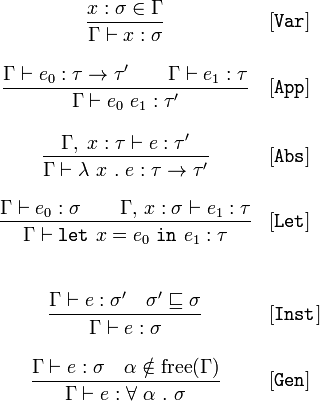
\includegraphics[width=80mm]{hindley-milner}
\end{figure}

Para explicar que quieren decir estas seis reglas primer es necesario entender la sintaxis y el significado de alguno de los símbolos.

Lo primero es la barra horizontal, esta viene a cumplir el rol de una implicación lógica, o sea, si el antecedente, lo de arriba, es verdadero entonces, necesariamente, el consecuente, lo de abajo, también lo es. Cuando en la parte superior hay N hipótesis, para asegurar el consecuente es necesario que se cumplan las N hipótesis, es como si las separaciones por espacio estubiesen indicando una operación and lógica.
Lo siguiente son los dos puntos \lstinline$":"$, estos indican de que tipo es una expresión, por ejemplo x : Int indica que x es del tipo int. El contexto se representa con $\gamma$. Para indicar que algo se encuentra en un determinado contexto usamos $\in$. $\vdash$ es básicamente que se puede demostrar algo, lo precede el contexto necesario para demostrar lo que quiere. La coma \lstinline$","$ es utilizada para ampliar el contexto, una unión, si entendemos al contexto como el conjunto de referencias a variables de determinados tipos, donde se pisa el elemento si este ya se encontraba en el contexto original. Por ultimo, el símbolo $\sqsubseteq$ indica una especie de inclusión, en realidad es mas bien una herencia, donde el tipo de la izquierda es un subtipo del de la derecha.
Con todos la notación clara es sencillo entender las seis reglas.
Por Ejemplo, la segunda indica que si en nuestro contexto tenemos una expresión e0 que  toma un elemento del tipo  $\tau$ y devuelve otro que es del tipo $\tau$', y en ese mismo entorno tenemos una segunda expresión que es del tipo $\tau$, entonces podemos decir que en ese mismo entorno que la expresión e0 e1 es del tipo $\tau$'.
La quinta nos dice que si en un entorno la expresión e es del tipo $\sigma$' y que $\sigma$' es un subtipo de $\sigma$ entonces la expresión e es del tipo  $\sigma$.

El algoritmo de inferencia de tipos usa estas reglas de forma recursiva. Realiza un ajuste de patrones, donde mira la expresión que tiene, y en cual de los consecuentes encaja mejor, una vez encontrado va a los antecedentes y mira que necesita para que estos se cumplen, si con la información actual es suficiente entonces ha terminado de inducir los tipos, en caso contrario toma estos antecedentes que aun no tiene determinados y vuelve a realizar el mismo ajuste de patrón, y así va infiriendo en cada sub-expresión los tipos necesarios. Cuando encuentra que la información alcanzada es suficiente para cumplir TODAS las hipótesis la inferencia esta completa.

\label{sub:algoritmo_de_hindley_milner}

\subsection{Ejemplo de aplicación del algoritmo} % (fold)
\label{sub:ejemplo_de_aplicaci_n_del_algoritmo}

Si hacemos el seguimiento del como funciona este algoritmo en la función sumar que tenemos más arriba, y utilizando la currificación de Haskell tenemos que la función es de la forma

\begin{lstlisting}
  sumar x y = x + y
\end{lstlisting}

que es lo mismo que

\begin{lstlisting}
  sumar x y = (+) x y
\end{lstlisting}

para ajustar el patrón tomamos

\begin{lstlisting}
  e0 = (+) x
  e1 = y
\end{lstlisting}

esto encaja en el segundo patrón, donde se realiza e0 e1 que es del tipo $\tau$', para esto se induce que e0 es del tipo $\tau$ $\rightarrow$ $\tau$' y que e1 es tipo $\tau$'. Hasta ahora solo sabemos que y es del tipo $\tau$.
Luego hay que ajustar el patrón e0. Donde volvemos a caer en el segundo caso. Entonces tenemos que :

\begin{lstlisting}
  e'0 = (+)
  e'1 = x
\end{lstlisting}

Con e'0 e'1 es del tipo $\tau$ $\rightarrow$ $\tau$'
Concluimos que, dado que e'0 es del tipo $\tau$1 $\rightarrow$ t1' y que e'1 es del tipo $\tau$1, como e'0 e'1 = e0
entonces e0 : $\tau$'1 = $\tau$ $\rightarrow$  $\tau$'
Hasta aquí tenemos que


\begin{lstlisting}[mathescape]
y : $\tau$
x : $\tau$1
(+) :  $\tau$1 $\rightarrow$  $\tau$ $\rightarrow$  $\tau$'
\end{lstlisting}

Además, como (+) : (Num a) => a $\rightarrow$ a $\rightarrow$ a
Por la primera regla tenemos que $\tau$1 $\rightarrow$  $\tau$ $\rightarrow$  $\tau$' = a $\rightarrow$ a $\rightarrow$ a
O sea

\begin{lstlisting}[mathescape]
$\tau$1 = a
$\tau$ = a
t' = a
\end{lstlisting}

Y, finalmente, usando la quinta regla tenemos que

\begin{lstlisting}[mathescape]
$\tau$1 $\sqsubseteq$ a
$\tau$ $\sqsubseteq$ a
t' $\sqsubseteq$ a
\end{lstlisting}

Finalmente solo resta recomponer todo, usando que sumar = e'0 e'1 e1
El tipo de sumar es (Num a) => a $\rightarrow$ a $\rightarrow$ a.

% subsection ejemplo_de_aplicaci_n_del_algoritmo (end)


  \section{Recursión} % (fold)
\label{sec:recursi_n}

La recursión o recursividad es la forma de especificar una función basandose
en su propia definición. Es una parte muy importante de Haskell. Una función
es recursiva cuando una parte de su definición incluye a la propia función.
Necesita por lo menos un \textit{caso base} que no hace llamado recursivo para
que exista una condición límite.

Este ejemplo muestra una función de factorial recursiva, separando
claramente el caso base.

\begin{lstlisting}
  factorial 0 = 1
  factorial n = n * factorial (n - 1)
\end{lstlisting}

Muchas de las funciones comunes en Haskell se pueden definir de forma
recursiva, por ejemplo el \textit{length}, la función que devuelve el
número de elementos de una lista:

\begin{lstlisting}
  length []     = 0
  length (x:xs) = 1 + length xs
\end{lstlisting}

Recursión es usada para definir casi todas las funciones de manejo de números
y listas, sin embargo en la práctica no es de usarse tan seguido: la
recursividad está abstraida por las funciones de las librerias de Haskell,
permitiendo al programador razonar sus problemas en más alto nivel. Por
ejemplo, la función de factorial de ejemplo escrita anteriormente se puede
definir de la siguiente manera:

\begin{lstlisting}
  factorial n = product [1..n]
\end{lstlisting}

% section recursi_n (end)


\section{Pereza} % (fold)
\label{sec:pereza}

Una característica destacable de Haskell es que es \textit{perezoso} (o
\textit{no estricto}). Esto significa que nada se va a evaluar hasta que sea
directamente necesario - la evaluación queda diferida hasta que el resultado
es requerido por otra computación.

El siguiente es un ejemplo de la pereza de Haskell:

\begin{lstlisting}
  let (a, b) = (length [1..5], reverse "hola mundo") in 1 + 1
\end{lstlisting}

Como la expresión después del \textit{in} no utiliza los valores de a y b,
estos quedan sin evaluar, ya que no son necesarios. Tambien pueden no ser
necesarios por completo, o ser \textit{parcialmente} requeridos:

\begin{lstlisting}
  let (a, b) = (length [1..5], reverse "hola mundo")
      'o':ss = b
\end{lstlisting}

Como solo es necesaria la primera letra para concluir el matcheo de
patrones, la evaluación es parcial.

Las funciones en Haskell pueden ser perezosas o estrictas. Podemos analizar
si una función es perezosa o estricta pasandole \lstinline$undefined$ y viendo
si su ejecución falla. Esto se debe a que en Haskell la evaluación forzada del
\lstinline$undefined$ siempre termina en un error.

\begin{lstlisting}
  let (x, y) = undefined in x  -- Error!
  length [undefined, undefined, undefined]
  -- No hay error, length es perezoso
\end{lstlisting}


La evaluación perezosa tiene muchas ventajas, pero su mayor inconveniente es
que el uso de memoria se vuelve muy dificil de predecir, por ejemplo las
expresiones \lstinline$3+2 :: Int$ y \lstinline$5 :: Int$ denotan el mismo
valor pero pueden tener diferentes tamaños en memoria.
% \singlespace

% \singlespace y
% section pereza (end)


  
\section{Garbage Collection} % (fold)
\label{sec:garbage_collection}

Muchos lenguajes implementan un Garbage Collection (GC) para ocuparse de los objetos no alcanzables y liberar dicha memoria.


Los lenguajes imperativos suelen generar una cantidad de basura a lo largo de su ejecución, y si estos constan de un GC simplifican la vida del programador, al desligarlo de la necesidad de liberar el espacio no utilizado, y de no deber perder nunca la referencia. De lo contrario, si un lenguaje posee un GC, el programador debe olvidarse de lo que no necesite, simplemente haciendolo inalcanzable, de este modo las referencias almacenadas son solos las que en ese momento resultan útiles, el GC pasará en algún momento y liberará la memoria no alcanzable.


Los lenguajes funcionales, como lo es Haskell, suelen generar muchísima mas basura que los lenguajes imperativos, esto es debido a la inmutabilidad de sus variables, y para guardar un nuevo valor es necesario crear una nueva variable. Cada iteración en un llamado recursivo genera un nuevo valor. En Haskell no es insólito producir 1Gb de datos en un segundo.
Para esto el compilador de Haskell GHC tiene un potente GC que se ocupa de gestionar la basura en forma eficiente.


La inmutabilidad de las variables en Haskell no solo obliga a generar gran cantidad de basura, sino que esta característica es aprovechada para realizar la recolección.
Para esto utiliza el criterio de generación: datos jóvenes y viejos. Las variables mas viejas, al ser inmutables, no apuntan nunca a un dato joven, pues los datos jóvenes no existen en el momento en que las variables viejas son creadas. Esta es la idea que utiliza el recolector de basura de Haskell para aumentar la eficiencia.
El recolector de basura no mirará toda la memoria en la que estuvo trabajando nuestro programa, sino que sólo revisará entre los valores más jóvenes, y liberará los que no estén señalados, que suelen ser la gran mayoría, dado el comportamiento recursivo. Esto también es una ventaja, porque en realidad, mientras mas basura joven aparezca menor es el trabajo que realiza el recolector de basura; esto, que resulta tan poco intuitivo se explica con la forma que se utiliza para almacenar los datos jóvenes y los viejos.
Los datos jóvenes son almacenados en un bloque de memoria especial, una “guardería”, cuando esta guardería se llena el GC mira sólo en esta memoria quienes son alcanzables, por lo tanto útiles y los copia en la memoria de las variables mas viejas, luego nos habilita a reutilizar la “guardería”, la cual se encuentra “vacía”, ya que cualquier dato que pisemos no será útil, o lo tendremos copiado con los valores mas viejos. Este es el motivo por el cual, con mayor cantidad de basura joven, la recolección es más rápida, lo que sucede es que hay menos datos que copiar.

% section garbage_collection (end)


  
\section{Funciones de orden superior} % (fold)
\label{sec:functiones_de_orden_superior}


Una función de orden superior es aquella que puede tomar funciones como parámetro, o devolver una función como resultado, o ambas cosas.

Haskell no solo soporta las funciones de orden superior, sino que hace un uso permanente de esta cualidad, y de forma muy natural.


\subsection{Funciones como parametro} % (fold)
\label{sub:funciones_como_parametro}

Una función que puede tomar como parámetro a otra función es considerada de orden superior. En Haskell esto se utiliza todo el tiempo para filtrar datos mediante algún criterio, realizar una acción sobre un conjunto de datos, etc.

Un ejemplo de una función que viene por defecto en Haskell que toma funciones como parámetro es la función filter, a la cual se le pasa una función y una lista, filter llama a la función con cada elemento de la lista, si la función devuelve true el elemento es añadido a la lista que da como resultado.

Si se implementa una función fQuickSort a la que le paso una función f que dado un elemento de la lista me devuelve un valor comparable, y una lista que quiero ordenar de la siguiente forma:

\begin{lstlisting}
fQuickSort :: (Ord b) => (a -> b) -> [a] -> [a]
fQuickSort _ [] = []
fQuickSort f (x:xs) =
  let
      menores = fQuickSort f [a | a <- xs, (f a) <= (f x)]
      mayores = fQuickSort f [a | a <- xs, (f a) > (f x)]
  in menores ++ [x] ++ mayores
\end{lstlisting}

En esta implementación es realmente versátil, ya que dependiendo que función f se utilice para medir el “tamaño” de los elementos de la lista obtendremos un resultado distinto, y no restringimos los elementos de la lista a elementos ordenables, dado que el criterio de orden los obtenemos en función de la “medida” de los elementos.

% subsection funciones_como_parametro (end)
\subsection{Funciones como resultado} % (fold)
\label{sub:funciones_como_resultado}

Dijimos que una función también es de orden superior si puede dar como resultado otra función. Esto es útil, pues se puede crear constructores de funciones, estos constructores recibirán un valor, y devolverán una función para cada valor que tomen. Por ejemplo:

\begin{lstlisting}
mutiplicarPor :: (Num a =>) a -> (a -> a)
multiplicarPor x = (*) x
\end{lstlisting}

Para cada valor de x, multiplicarPor da como resultado una función que recibe un numero y devuelve el el producto del numero pasado con x.


En realidad, Haskell utiliza las funciones de orden superior todo el tiempo, ya que las funciones de Haskell solo pueden tomar una única variable, esto es lo mismo que decir que las funciones en Haskell están Currificadas. No hay ninguna contradicción, cuando tenemos una función que aparenta recibir más de una variable lo que en realidad tenemos es una función que recibe un dato y nos devuelve una función, la cual toma el siguiente dato, y nos devuelve otra función y así sucesivamente. Esta es la explicación del porque cuando anotamos en la definición de tipos de una función no diferenciamos entre los parámetros de entrada y el valor de retorno.

La Currificación hace evidente la necesidad de que el lenguaje soporte funciones de orden superior. A medida que vamos aplicando parcialmente la función vamos obteniendo nuevas funciones como resultado, y este es el concepto de que una función sea de orden superior por devolver una función. Usando el ejemplo anterior, el fQuickSort es un constructor de sorts, al que se le pasa una función f y nos da un sort que ordena con un determinado criterio, lo mismo pasa con filter y map.

\begin{lstlisting}
sumar3 x y z = x + y + z
\end{lstlisting}

\begin{lstlisting}
ghci> :t sumar3
sumar3 :: forall a. Num a => a -> a -> a -> a
ghci> :t sumar3 1
sumar3 1 :: forall a. Num a => a -> a -> a
ghci> :t sumar3 1 2
sumar3 1 2 :: forall a. Num a => a -> a
ghci> :t sumar3 1 2 3
sumar3 1 2 3 :: forall a. Num a => a
ghci> :t 6
6 :: forall a. Num a => a
\end{lstlisting}

En Haskell este tipo de funciones son tan comunes que tiene montones de aplicaciones en las librerías standar utilizando funciones de orden superior, ya mencionamos las funciones  filter y map, pero se incluyen muchos más.

% subsection funciones_como_resultado (end)

\subsection{Plieges (folds)} % (fold)
\label{sub:plieges_}

Unas funciones particularmente útiles y cómodas son los pliegues (folds).
Como en Haskell las variables son inmutables no existen los iteradores clásicos de los lenguajes imperativos, sino que se utiliza la recursividad de las funciones, esto es tan común que existen algunas funciones útiles tienen incorporado estos patrones para realizar iteraciones. Si querríamos implementar la función elem utilizando pliegues podríamos hacerlo como

\begin{lstlisting}
elem' :: (Eq a)=> a -> [a] -> Bool
elem' y ys = foldl f False ys
  where f acc x = if x==y then True else acc
\end{lstlisting}

Lo que estamos haciendo es pasarle a nuestro pliegue una función que devuelve True si el elemento que recibe es el mismo que el que nosotros buscamos, y sino devuelve el acc, además la función recibe como “segundo” parámetro el valor inicial del acumulador que va a pasarle a la función, y una lista sobre la que deseamos que itere. Lo que hace foldl es agarrar la cabeza de la lista, pasarselo a la función f, y tomar el valor obtenido como nuevo acumulador, luego se llama a si mismo con la cola de la lista, la misma función y este nuevo acumulador. El resultado que devuelve foldl es el ultimo valor que devuelve el acumulador.

Si quisiéramos implementar foldl podríamos hacerlo así:

\begin{lstlisting}
foldl' :: (a->b->a)-> a->[b]->a
foldl' _ acc [] = acc
foldl' f acc (x:xs) = foldl' f (f acc x) xs
\end{lstlisting}

% subsection plieges_ (end)


\subsection{Funciones Anónimas (lambdas)} % (fold)
\label{sub:funciones_an_nimas_}


Al usar este tipo de funciones solemos tener que crear funciones con el único objetivo de pasarlas a nuestras funciones de orden superior, lo cual no tiene mucho sentido, para esto aparecen las denominadas funciones anónimas, o funciones lambdas. Las funciones lambda son expresiones (devuelven un valor), por eso podemos pasarlas como parámetros a funciones de orden superior.
Su sintaxis es:

\begin{lstlisting}
(\a b -> 2a/b)
\end{lstlisting}

donde a y b son los parámetros que recibe, lo que sucede a  -> indica que el comportamiento de dicha función. Suelen estar encerradas entre paréntesis para delimitarlas, de lo contrario tomarán todo el renglón.
Utilizando este tipo de funciones, podríamos haber escrito nuestro pliegue como

\begin{lstlisting}
elem' :: (Eq a)=> a -> [a] -> Bool
elem' y ys = foldl (\acc x-> if x==y then True else acc) False ys
\end{lstlisting}

% subsection funciones_an_nimas_ (end)

% section functiones_de_orden_superior (end)


  \section{Módulos} % (fold)
\label{sec:m_dulos}

Los módulos son colecciones de tipos, clases de tipos y funciones relacionadas entre sí.
En un programa hecho en Haskell, el módulo principal carga otros módulos y utiliza las funciones de los mismos para realizar lo que el programa fuere a hacer.
Es una buena práctica programar dividiendo el código en módulos lo mas independiente posibles para tener un mejor mantenimiento del programa y aprovechar código que puede ser reutilizado.

\subsection{Sintaxis} % (fold)
\label{sub:sintaxis}
La sintaxis para importar módulos en Haskell es \lstinline$import <modulename>$, y las importaciones de los módulos suelen estar al principio de los ficheros ya que deben realizarse antes de definir cualquier función.

Una vez que se importan los módulos, pasan a estar definidos en el espacio global.
Hay varias maneras de importar un módulo. A continuación veremos ejemplos importando el módulo \textbf{Data.List}, el cual contiene funciones para el manejo de listas:

Si se quiere importar todo el módulo:

\begin{lstlisting}
import Data.List
\end{lstlisting}

Para importar algunas funciones del módulo (en este caso las funciones intercalate y sort del módulo \textbf{Data.List}):

\begin{lstlisting}
import Data.List (intercalate, sort)
\end{lstlisting}

Para importar todo el módulo excepto una o más funciones (en este caso todo el módulo Data.List excepto sus funciones intercalate y sort):

\begin{lstlisting}
import Data.List hiding (intercalate, sort)
\end{lstlisting}

Importaciones cualificadas (para evitar colisiones de nombres):

\begin{lstlisting}
import qualified Data.Map
\end{lstlisting}

En este caso, si queremos referirnos, por ejemplo, a la función filter de \textbf{Data.Map}, debemos utilizar \textbf{Data.Map.filter}, mientras que si usamos simplemente filter nos referimos al filtro normal que utiliza Haskell.

Una manera más fácil de hacer llamadas a módulos importados de manera cualificada es renombrar al módulo de manera que la llamada sea más abreviada:

\begin{lstlisting}
import qualified Data.Map as M
\end{lstlisting}

De esta manera, si yo quiero llamar a la función filter de \textbf{Data.Map}, debo utilizar simplemente \textbf{M.filter}. Algunos módulos que vienen con Haskell:

\begin{itemize}
  \item Para listas: \textbf{Data.List}
  \item Para caracteres: \textbf{Data.Char}
  \item Para listas de asociación (listas de duplas (\"clave\", \"valor\") ): \textbf{Data.Map}
  \item Para conjuntos: \textbf{Data.Set}
\end{itemize}
% subsection sintaxis (end)

\subsection{Creación de módulos} % (fold)
\label{sub:creaci_n_de_m_dulos}

Para crear un módulo, lo definimos en el script y dentro del módulo definimos sus funciones (utilizando la construcción \textbf{where}):

\begin{lstlisting}
module Areas
( areaCirculo
, areaCuadrado
, areaRectangulo
) where

areaCirculo :: Float -> Float
areaCirculo radio = pi * (radio ^ 2)

areaCuadrado :: Float -> Float
areaCuadrado lado = lado ^ 2

areaRectangulo :: Float -> Float -> Float
areaRectangulo a b = a * b
\end{lstlisting}

Para importarlo en otro script, se hace como se mencionó anteriormente (Areas está en el mismo directorio donde estamos trabajando):

\begin{lstlisting}
import Areas

areaCirculo 1.0
areaCuadrado 2.0
areaRectangulo 3.0 1.0
\end{lstlisting}


% subsection creaci_n_de_m_dulos (end)

% section m_dulos (end)


  \section{Functores} % (fold)
\label{sec:functores}

Los functores son una clase de tipos que tiene un método llamado fmap, donde

\begin{lstlisting}
fmap :: (a -> b) -> f a -> f b
\end{lstlisting}

La idea de fmap es que toma una funcion de a en b, un functor que contiene un a, y devuelve un functor que tiene un b. Una idea intuitiva de un functor podría ser como una caja, fmap abre esta caja, aplica f al contenido y devulve una caja con el resultado de aplicar la función.

Un término más correcto para definir lo que es un funtor sería contexto computacional. El contexto sería que la computación podría tener un valor, o podría fallar. Si queremos un constructor de tipos que sea una instancia de functor este debe pertenecer a la familia \lstinline$* -> *$.

Algunos functores básicos son las listas [], Maybe, Either a (en este ultimo caso, como necesitamos que nuestro tipo tome un único tipo concreto y Either toma dos debe estar parcialmente evaluda), si se definiese una clase Tree a también podría ser un funtor. Otros no tan claros son IO y (->) r.

Las acciones IO son como cajas que encierran datos que provienen del mundo real, o que saldrán al mismo, podemos ligar el contenido de una acción IO a una variable usando <-, trabajar con estos datos, realizar algunos calculos, pero cuando querramos sacarlos al mundo exterior es necesario transformarlos en otra acción IO usando return. Si queremos mapear un valor IO  lo que en realidad buscamos es obtener una nueva acción IO que contenga el resultado de aplicar una determinada función, esto será:

\begin{lstlisting}
instance Functor IO where
  fmap f action = do
    result <- action
    return (f result)
\end{lstlisting}

El tipo de una función r -> a se puede reescribir como (->) r a esto indica que (->) r es una caja de a. Como -> es de la familia \lstinline$* ->  * -> *$ debe estar parcialmente aplicado, igual que Either.

\begin{lstlisting}
instance Functor ((->) r) where
  fmap f g = (\x -> f (g x))
\end{lstlisting}

Aplicar fmap a una función nos da una nueva función, si pensamos que aplicamos esta nueva funcion a un valor esto daría por resultado la función original aplicada a nuestro valor, y a este resultado le aplicaría la función que le pasamos a fmap, esto no es otra cosa que realizar la composición de funciones.

\begin{lstlisting}
instance Functor ((->) r) where
  fmap = (.)
\end{lstlisting}

\subsection{Leyes de los Functores} % (fold)
\label{sub:leyes_de_los_functores}


Ahora vamos a ver las leyes de los functores. Para que algo sea una functor, debe satisfacer una serie de leyes. Se espera que todos los functores exhiban una serie de propiedades y comportamientos. Deben comportarse fielmente como cosas que se puedan mapear. Al llamar fmap sobre un functor solo debe mapear una función sobre ese funtor, nada más. Este comportamiento se describe en las leyes de los functores. Hay dos de ellas que todas las instancias deFunctor deben cumplir, pero Haskell no hace esta comprobación, debe ser verificada por el usuario que la implementa.

La primera ley de funtores establece que si mapeamos la función identidad sobre un functor, el functor que obtenemos debe ser igual que el original (fmap id = id).

La segunda ley dice que si mapeamos el resultado de una composición de dos funciones sobre un funtor debe devolver lo mismo que si mapeamos una de estas funciones sobre el funtor inicial y luego mapeamos la otra función \lstinline$((f . g) = fmap f)$

% subsection leyes_de_los_functores (end)

\subsection{Functores Aplicativos} % (fold)
\label{sub:functores_aplicativos}


Dentro de un functor podemos tener almacenado cualquier tipo de valor, y como en Haskell las funciones son ciudadanos de primer orden estas también son un valor, por ende podemos tener funciones encerradas dentro de un functor, por ejemplo, si hacemos

\begin{lstlisting}
fmap (*) Just 7
\end{lstlisting}

obtenemos

\begin{lstlisting}
Just (* 7)
\end{lstlisting}

Si queremos aplicar la función almacenada a el valor almacenado por Just 11 podriamos tratar de hacerlo, pero si queremos un comportamiento que funcione en todos los functores debemos crear algo más general, este es el motivo por el cual aparecen los functores aplicativos.

\begin{lstlisting}
class (Functor f) => Applicative f where
  pure :: a -> f a
  (<*>) :: f (a -> b) -> f a -> f b
\end{lstlisting}

La definición de esta clase de tipos nos dice que si alguien es un Applicativa también es un Functor.
Las funciones no están implementadas por defecto, pero pure toma un valor y lo encapsula dentro de un functor aplicativo.
La segunda funcion es una ampliacion de fmap, toma un functor aplicativo, “extrae” su función, y mapea dicha función sobre otro functor. La clase de tipos maybe los implementa de la sigueinte forma:

\begin{lstlisting}
instance Applicative Maybe where
  pure = Just
  Nothing <*> _ = Nothing
  (Just f) <*> something = fmap f something
\end{lstlisting}

% subsection functores_aplicativos (end)

% section functores (end)


  \section{Mónadas} % (fold)
\label{sec:m_nadas}

Las \textbf{mónadas} en Haskell se pueden pensar como descripciones
\textit{componibles} de computaciones. Presentan la posibilidad de separar la
combinación de computaciones de su ejecución y permiten acarrear datos extra
implícitamente en adición al resultado de la computación, que
\textit{se producirá} cuando la mónada sea corrida. De esta manera permiten
suplementar las funcionalidades \textit{puras} con I/O, estado, indeterminismo,
etc.

En terminos del lenguaje una mónada es un tipo parametrizado que es instancia
de la clase \textit{Monad}. Su definición es la siguiente:

\begin{lstlisting}
class Monad m where
    return :: a -> m a
    (>>=) :: m a -> (a -> m b) -> m b
    (>>) :: m a -> m b -> m b
\end{lstlisting}

Podemos ver la mónada como un contenedor para un valor \textbf{a}. La función
\lstinline$return$ se ocupa de poner ese valor adentro de la mónada. Entonces
la función \lstinline$(>>=)$, tambien conocida como \textit{bind}, aplica la
función que se le pasa por parámetro al contenido de la mónada obteniendo como
resultado otra mónada (obviamente la función pasada tiene que tener el tipo
adecuado). Se puede ver como funciona en el siguiente ejemplo:

\begin{lstlisting}
putStrLn "Como te llamas?"
>>= (\_ -> getLine)
>>= (\name -> putStrLn ("Hola, " ++ name ++ "!"))
\end{lstlisting}

El operador \lstinline$(>>=)$ se ocupa de tomar el valor del lado izquierdo
y combinarlo con la función del lado derecho para producir un valor nuevo. El
ejemplo de arriba se puede reescribir con la notación \lstinline$do$, que es un
azucar sintáctico alrededor del operador \textit{bind}:

\begin{lstlisting}
do
   putStrLn "Como te llamas?"
   name <- getLine
   putStrLn ("Hola, " ++ name ++ "!")
\end{lstlisting}

Ese código puede parecer de un lenguaje imperativo, y de hecho lo es: otra
forma de ver las mónadas es pensar que son la abstracción necesaria para
suplementar las funcionalidades que no cuadran adentro del paradigma funcional.

La implementación mas sencilla del \lstinline$(>>=)$. toma el valor del lado
izquierdo, le aplica la función y devuelve el resultado, sin embargo se vuelve
realmente útil cuando esa implementación hace algo extra.

\subsection{Las Leyes de las Mónadas} % (fold)
\label{sub:las_leyes_de_las_m_nadas}

Las mónadas por convención deben cumplir las siguientes leyes:

\begin{lstlisting}
  -- Identidad por la izquierda
  return x >>= f = f x

  -- Identidad por la derecha
  m >>= return = m

  -- Asociatividad
  (m >>= f) >>= g = m >>= (x -> f x >>= g)
\end{lstlisting}

Para poder entenderlo mejor y usarlo de una forma más sencilla, el módulo
Control.Monad define el operador de composición de mónadas:

\begin{lstlisting}
(>=>) :: Monad m => (a -> m b) -> (b -> m c) -> a -> m c
(m >=> n) x = do
                  y <- m x
                  n y
\end{lstlisting}

Con el uso de ese operador las tres reglas pueden escribirse de la siguiente
forma:

\begin{lstlisting}
  -- Identidad por la izquierda
  return >=> f = f

  -- Identidad por la derecha
  f >=> return = f

  -- Asociatividad
  (f >=> g) >=> h = f >=> (g >=> h)
\end{lstlisting}

% subsection las_leyes_de_las_m_nadas (end)

\subsection{Mónadas comunes} % (fold)
\label{sub:m_nadas_comunes}

La siguiente tabla lista las mónadas más comunes usadas en Haskell, denotando
el problema que tratan de solucionar en términos imperativos.
\linebreak
\begin{tabular}{ | p {3cm} | p {5cm} |}
  \hline
  Mónada & Semántica imperativa \\
  \hline
  \hline
  Maybe & Excepción anónima \\
  \hline
  Error & Excepción con descripción \\
  \hline
  State & Estado global \\
  \hline
  IO & Entrada y Salida \\
  \hline
  [] (list) & Indeterminismo \\
  \hline
  Reader & Entorno \\
  \hline
  Writer & Logger \\
  \hline
\end{tabular}

En las siguientes secciones se explicarán algunas de las mónadas que aparecen
en esta tabla.
% subsection m_nadas_comunes (end)


\subsection{Manejo de errores} % (fold)
\label{sub:manejo_de_errores}


\subsubsection{Mónada Maybe} % (fold)
\label{ssub:m_nada_maybe}

Es una de las mónadas más utilizadas y es muy sencilla a la vez. La definición
de esta Mónada es la siguiente:

\begin{lstlisting}
data Maybe a = Nothing | Just a

instance Monad Maybe where
    return         = Just
    fail           = Nothing
    Nothing  >>= f = Nothing
    (Just x) >>= f = f x
\end{lstlisting}

La mónada Maybe incorpora la posibilidad de encadenar computaciones que pueden
devolver Nothing como resultado, en cuyo caso la cadena terminaría antes. Por ejemplo:

\begin{lstlisting}
maybeHalf :: Int -> Maybe Int
maybeHalf a
         | even a = Just (div a 2)
         | otherwise = Nothing
\end{lstlisting}

La función que acabamos de definir devolverá la mitad de un número, si es par, y \textbf{Nothing} si es impar. La podemos usar de la siguiente manera:

\begin{lstlisting}
ghc> Just 10 >>= maybeHalf
Just 5
ghc> Just 10 >>= maybeHalf >>= maybeHalf
Nothing
ghc> Just 10 >>= maybeHalf >>= maybeHalf >>= maybeHalf
Nothing
\end{lstlisting}

Sin el uso de la mónada Maybe nos veriamos obligados a anidar if y else para las llamadas consecutivas.

\subsubsection{Either} % (fold)
\label{ssub:either}

Otra mónada muy usada es \textit{Either}. Su tipo está definido de la
siguiente manera:

\begin{lstlisting}
data Either a b = Left a | Right b
\end{lstlisting}

Su propósito es muy parecido al de Myabe, Left es considerado un error
mientras que Right - un valor normal. La diferencia es que Left permite
guardar un valor (a diferencia del Nothing en el caso de Maybe).

Podemos escribir una función que divida un número por una lista de enteros uno por uno segura utilizando \textbf{Either}:

\begin{lstlisting}
divBy :: Integral a => a -> [a] -> Either String [a]
divBy _ [] = Right []
divBy _ (0:_) = Left "divBy: division by 0"
divBy numerator (denom:xs) =
    case divBy numerator xs of
      Left x -> Left x
      Right results -> Right ((numerator `div` denom) : results)
\end{lstlisting}

Y la podemos utilizar de la siguiente forma:

\begin{lstlisting}
ghci> divBy 50 [1,2,5,8,10]
Right [50,25,10,6,5]
ghci> divBy 50 [1,2,0,8,10]
Left "divBy: division by 0"
\end{lstlisting}

% subsubsection _ither (end)


\subsubsection{Mónada Error} % (fold)
\label{ssub:m_nada_error}

La mónada Error es la forma que tiene Haskell de simular las
\textit{excepciones}. Se logra de la siguiente forma: se encadenan
computaciones que pueden lanzar excepción derivando la ejecución a la
instancia que puede manejarla. Esta es la definición de \textbf{MonadError}:

\begin{lstlisting}
class Monad m => MonadError e m | m -> e where
    throwError :: e -> m a
    catchError :: m a -> (e -> m a) -> m a
\end{lstlisting}

Un ejemplo de uso es:

\begin{lstlisting}
example :: (Error e, MonadError e m) => m String
example = throwError (strMsg "Esto es un error")
    `catchError` const (return "Atrapo el error")

example >>= putStrLn        -- Imprime "Atrapo el error"
\end{lstlisting}

Note que el tipo MonadError lleva 2 parametros, \textbf{e}, el tipo de error, y \textbf{m}, constructor que representa una mónada. Mas adelante en la definición se ve que el \textbf{throwError} y \textbf{catchError} son métodos de la clase MonadError, siendo los equivalentes a las estructuras familiares de otros lenguajes. Eso tiene la ventaja de poder definir su significado para cada mónada particular.

% subsection m_nada_error (end)

% subsection manejo_de_errores (end)

\subsection{Mónada List} % (fold)
\label{sub:m_nada_list}


Resulta que la lista es una mónada tambien! Las listas se utilizan para modelar
las computaciones no determinísticas que pueden devolver un número de
resultados arbitrario. Se define de la siguiente manera:

\begin{lstlisting}
instance Monad [] where
    m >>= f  = concat (map f m)
    return x = [x]
\end{lstlisting}

El return es fácil de entender: simplemente devuelve una lista de un elemento.
El operador \textit{bind} tambien se entiende si consideramos que tiene que
cumplir con el tipo \lstinline$[a] -> (a -> [b]) -> [b]$ (por su defenición
más general). La función \textbf{f} aplica a cada elemento y, dado su tipo,
retorna una lista - por eso es necesario el \lstinline$concat$ al final, para
a la salida obtener una lista.

¿Por qué las listas son mónadas? Se explica con el siguiente ejemplo de
notación monádica de una lista:

\begin{lstlisting}
foo = do
  x <- [1 .. 10]
  y <- [2, 3, 5, 7]
  return (x * y)
\end{lstlisting}

\textbf{foo} es un múltiplo de x e y, con x siendo un número no determinístico
entre 1 y 10, e y siendo 2, 3, 5 o 7. Este ejemplo es la notación larga y
monádica de una comprensión de lista, podría ser escrita así:

\begin{lstlisting}
foo = [x * y | x <- [1 .. 10], y <- [2, 3, 5, 7]]
\end{lstlisting}
% subsection m_nada_list (end)


\subsection{Mónada IO} % (fold)

Dado que Haskell es un lenguaje funcional y perezoso, no podemos expresar las
efectos reales de las operaciones de entrada y salida con funciones puras. De
hecho, estas operaciones no se pueden ejecutar perezosamente, ya que esto
haria que los efectos reales sean impredecibles. La mónada \textbf{IO} es el
medio para representar las acciones de entrada/salida como valores de Haskell,
para que el programador pueda manipularlos con funciones puras.


\label{sub:m_nada_io}

% subsection m_nada_io (end)


\subsection{Mónada State} % (fold)
\label{sub:m_nada_state}

La mónada \textit{State} permite acarrear estado a lo largo de una ejecución.
Con ella se puede hacer lo siguiente: dado un valor de estado, se produce un
resultado y un nuevo valor de estado. Esta es su definición:

\begin{lstlisting}
newtype State s a = State { runState :: (s -> (a,s)) }

instance Monad (State s) where
  return x = State $ \s -> (x,s)
  (State h) >>= f = State $ \s -> let (a, newState) = h s
                                      (State g) = f a
                                  in  g newState
\end{lstlisting}

Como se ve en la declaración de tipo, State es solo una abstracción
de una función que toma un estado, devuelve un valor intermedio y un nuevo
estado.

Un ejemplo de uso de State es una pila. La función \textbf{push}
agrega un elemento al tope de la pila y \textbf{pop} saca uno. Sin State
tendriamos que arrastrar la pila como argumento a estas funciones, lo cual
no es lo más cómodo de usar. Con State la podemos definir de la siguiente
forma:

\begin{lstlisting}
type Stack = [Int]

pop :: State Stack Int
pop = State $ \(x:xs) -> (x,xs)

push :: Int -> State Stack ()
push a = State $ \xs -> ((),a:xs)
\end{lstlisting}

Un ejemplo de uso de la pila sería:

\begin{lstlisting}
stackManip = do
    push 3
    a <- pop
    pop
\end{lstlisting}

La implementación de State en Control.Monad también es instancia de la clase
MonadState que define 2 funciones muy útiles:

\begin{lstlisting}
put newState = State $ \_ -> ((), newState)
get = State $ \st -> (st, st)
\end{lstlisting}

Las cuales nos permiten manejar el estado de una manera más sencilla.

% subsection m_nada_state (end)

\subsection{Mónada Reader} % (fold)
\label{sub:m_nada_reader}

Algunos problemas de programación requieren computaciones en un cierto entorno (como un set de variables), pero no requieren la generalidad de la mónada \textbf{State}. La mónada \textbf{Writer} permite aportarle a una computación un entorno. Esta es su definición de tipo y su instancia de mónada:

\begin{lstlisting}
newtype Reader r a = Reader {  runReader :: r -> a }

instance Monad (Reader e) where
    return a         = Reader $ \e -> a
    (Reader r) >>= f = Reader $ \e -> runReader (f (r e)) e
\end{lstlisting}

En el siguiente ejemplo se puede ver facilmente su utilidad:

\begin{lstlisting}
import Control.Monad.Reader

greeter :: Reader String String
greeter = do
    name <- ask
    return ("Hola, " ++ name ++ "!")
\end{lstlisting}

\begin{lstlisting}
ghci> runReader greeter "Jorge"
"Hola, Jorge!"
\end{lstlisting}

Usamos la función \textbf{ask} que esta definida en la clase \textbf{MonadReader}. Esta es su definición y el como Reader implementa esa clase:

\begin{lstlisting}
class MonadReader e m | m -> e where
    ask   :: m e
    local :: (e -> e) -> m a -> m a

instance MonadReader (Reader e) where
  ask       = Reader id
  local f c = Reader $ \e -> runReader c (f e)
\end{lstlisting}

Esta clase provee de funciones para que el uso de \textbf{Reader} sea más cómodo. \textbf{ask} recupera el entorno y \textbf{local} ejecuta la computación en el entorno modificado.

% subsection m_nada_reader (end)

\subsection{Mónada Writer} % (fold)
\label{sub:m_nada_writer}

La mónada \textbf{Writer} sirve para producir un stream de datos adicional a los valores computados.
Es útil para generar un log sobre una ejecución.
Esta es la definición del tipo \textbf{Writer}. Como con los ejemplos anteriores, nos permite redefinir su comportamiento:

\begin{lstlisting}
newtype Writer w a = Writer { runWriter :: (a, w) }
\end{lstlisting}

A continuación se puede ver un ejemplo sencillo de uso del Writer:

\begin{lstlisting}
import Control.Monad.Writer

doubleWithLog :: Int -> Writer String Int
doubleWithLog x = do
        tell ("Acabo de duplicar " ++ (show x) ++ "!")
        return (x * 2)
\end{lstlisting}

Si ejecutamos esta función, obtendremos lo siguiente:

\begin{lstlisting}
ghci> runWriter $ doubleWithLog 8
(16, "Acabo de duplicar 8!")
\end{lstlisting}

% subsection m_nada_writer (end)


% section m_nadas (end)


  \section{Zippers} % (fold)
\label{sec:zippers}

Los zippers tienen como objetivo lograr un movimiento de forma eficiente en una estructura, conocida, que almacena datos. En un zipper se almacena el dato al que se ha llegado por un movimiento y, además, la información necesaria para reconstruir toda la estructura original.

Un problema muy sencillo para ver la utilidad de los zippers es el de querer aplicar una función en una hoja de un árbol, y luego aplicar la misma función en el hermano de dicha hoja. Si no se contase con una estructura del tipo zipper, habría que realizar todo el recorrido hasta la hoja, luego aplicar la función, y luego volver, desde la raíz a realizar el mismo recorrido, salvo en el último movimiento, y nuevamente aplicar la función. Usando los zippers podemos movernos hasta la hoja deseada, y como podemos reconstruir la estructura, podemos pedir el padre, y además saber si el nodo actual era el hijo izquierdo o el derecho, para así saltar al nodo hermano y aplicar nuevamente la función.
Con este ejemplo se observa que al querer realizar determinadas acciones con bloques de información de una estructura, y estos datos se encuentran “próximos” en dicha estructura, al construir un zipper para esta estructura nos ahorramos recorrer reiteradas veces la estructura original, mejorando la velocidad de nuestro programa.

Volviendo al ejemplo del árbol binario podemos definir las estructuras de la siguiente forma:

\begin{lstlisting}
data Tree a = Empty | Node a (Tree a) (Tree a) deriving (Show)
data Crumb a = LeftCrumb a (Tree a) | RightCrumb a (Tree a) deriving (Show)
type Breadcrumbs a = [Crumb a]

type Zipper a = (Tree a, Breadcrumbs a)
\end{lstlisting}

Aquí se crea el tipo árbol, el cual puede estar vacío o tener un dato y otros dos árboles. El tipo miga, el cual dice si nos movimos a la derecha o a la izquierda, contiene la información que contenía el nodo padre, y además tiene el subárbol  no visitado. Además se crea el sinónimo de tipo migas de pan, que simplemente es una lista de migas. Por ultimo se crea el tipo zipper, el cual tiene el árbol en el cual estaremos parados, y además las migas de pan del camino recorrido.
Con todos estos tipos de datos definidos podemos crear funciones que nos permitan movernos por de forma adecuada por los árboles.

\begin{lstlisting}
goUp :: (Tree a, Breadcrumbs a) -> (Tree a, Breadcrumbs a)
goUp (t, LeftCrumb x r:bs) = (Node x t r, bs)
goUp (t, RightCrumb x l:bs) = (Node x l t, bs)

goRight :: (Tree a, Breadcrumbs a) -> (Tree a, Breadcrumbs a)
goRight (Node x l r, bs) = (r, RightCrumb x l:bs)

goLeft :: (Tree a, Breadcrumbs a) -> (Tree a, Breadcrumbs a  )
goLeft (Node x l r, bs) = (l, LeftCrumb x r:bs)
\end{lstlisting}

Con estas tres funciones podemos movernos libremente, y eficientemente, sobre el árbol. Si una vez alcanzada una determinada posición queremos realizar un cambio sobre ese árbol podemos usar la siguiente función

\begin{lstlisting}
modify :: (a -> a) -> Zipper a -> Zipper a
modify f (Node x l r, bs) = (Node (f x) l r, bs)
modify f (Empty, bs) = (Empty, bs)
\end{lstlisting}

Esta función recibirá una función y un zipper, y nos devolverá un nuevo zipper, el cual es el resultado de aplicarle la función al nodo actual. Además podrían crearse otras funciones útiles, por ejemplo, una función que reciba un árbol y devuelva un zipper de dicho árbol, utilizando el árbol pasado como la raíz, una función que dado un zipper indique si se puede subir, o estamos en la raíz del árbol, otra que agregue/reemplace un subárbol por otro que le pasemos, otra que se ocupe de llegar a la raíz, etc.

Otra estructura, más sencilla, en la que son útiles los zippers son las listas, donde los movimientos posibles serían avanzar o retroceder:

\begin{lstlisting}
type ListZipper a = ([a],[a])

goForward :: ListZipper a -> ListZipper a
goForward (x:xs, bs) = (xs, x:bs)

goBack :: ListZipper a -> ListZipper a
goBack (xs, b:bs) = (b:xs, bs)
\end{lstlisting}

La primera lista del zipper es la cola de la lista original que resulta del movimiento, la segunda es una lista invertida de los elementos que están por delante del elemento actual. En este caso los zippers son mas simples que en los árboles, pero no por esto dejan de ser útiles. En Haskell los Strings son un sinónimo de tipo de una lista de caracteres, o sea que podemos usar un zipper para movernos dentro de un texto, y modificar y o agregar caracteres en el mismo, esto es realmente útil si estamos creando un editor de texto.

% section zippers (end)


  

\section{Concurrencia} % (fold)
\label{sec:concurrencia}


Un programa concurrente necesita realizar varias tareas al mismo tiempo. Estas tareas no necesariamente tienen que estar relacionadas entre si. El correcto funcionamiento de un programa concurrente no necesita varios núcleos.

En contraste, un programa paralelo soluciona un solo problema con el mejor rendimiento posible, empleando para eso más de un núcleo.

\subsection{Threads} % (fold)
\label{ssub:threads}

Un hilo es una acción \textit{IO} que se ejecuta independientemente de los otros hilos. Los hilos en Haskell no son determinísticos.
Para crear un thread, usamos la función \textit{forkIO} del módulo \textit{Control.Concurrent}.

Un ejemplo de uso podría ser la compresión de un archivo:

\begin{lstlisting}
import Control.Concurrent (forkIO)
import qualified Data.ByteString.Lazy as L
import Codec.Compression.GZip (compress)

compressFile = L.writeFile "files/foo.gz" . compress

do
    content <- L.readFile "files/foo.txt"
    forkIO (compressFile content)
    putStrLn "Gracias por comprimir!"
    return ()
\end{lstlisting}

% subsubsection threads (end)

\subsection{Comunicación entre hilos} % (fold)
\label{ssub:comunicaci_n_entre_hilos}

La forma más simple que tiene un hilo para comunicarse con otro es compartiendo una variable. En Haskell podemos lograrlo utilizando una variable sincronizable \textbf{MVar}. Una \textbf{MVar} actúa como una caja con un solo elemento, que puede estar vacia o llena. Si tratamos de poner un valor adentro de una \textbf{MVar} que ya está llena, la ejecución del hilo en cuestión se suspenderá hasta que otro hilo la vacie. De la misma manera, si intentamos sacar el valor de una \textbf{MVar} vacia, el hilo se suspenderá hasta que algún otro thread le agregue algo. En el siguiente ejemplo se puede ver el uso de una \textbf{MVar}:

\begin{lstlisting}
import Control.Concurrent

do
  m <- newEmptyMVar
  forkIO $ do
    v <- takeMVar m
    putStrLn ("Recibido " ++ show v)
  putStrLn "Enviando"
  putMVar m "Hola!"
\end{lstlisting}

Utilizamos la función \textit{newEmptyMVar} para crear una MVar, \textit{putMVar} para ponerle un valor adentro y \textit{takeMVar} para sacarlo. Notese que solo podemos utilizar una MVar adentro de un bloque \textit{do}.

% subsubsection comunicaci_n_entre_hilos (end)

\subsection{Comunicación por canales} % (fold)
\label{ssub:comunicaci_n_por_canales}

Utilizando el tipo \textit{Chan}, podemos crear una comunicación mediante un canal. El siguiente código ejemplifica su uso:

\begin{lstlisting}
import Control.Concurrent
import Control.Concurrent.Chan

do
  ch <- newChan
  forkIO $ writeChan ch "Hola!"
  forkIO $ writeChan ch "Hola desde otro hilo!"
  readChan ch >>= print
  readChan ch >>= print
\end{lstlisting}

Si el \textit{Chan} está vacio, el bloque \textit{readChan} espera hasta que haya un valor para leer. La función \textit{writeChan} nunca se bloquea, escribe al canal inmediatamente.

% subsubsection comunicaci_n_por_canales (end)

\subsection{Aclaraciones y problemas} % (fold)
\label{ssub:aclaraciones_y_problemas}

Para tener en cuenta: \textbf{MVar} y \textbf{Chan} no son \textit{estrictos}, su contenido no es evaluado sin explicitarlo. Además, el \textbf{writeChan} siempre acepta lo que se le escribe. Si un hilo escribe más frecuentemente que otro lee los mensajes, el canal crecerá desatendidamente.

Ambos métodos de comunicación entre hilos sufren de una serie de problemas típicos de concurrencia de estado compartido (en el caso de \textit{Chan} se debe a que internamente están implementados con Mvars). Los problemas más conocidos son \textit{deadlock} y \textit{starvation}. En una situación de \textit{Deadlock} dos o más hilos quedan suspendidos para siempre esperando el acceso a un recurso compartido. \textit{Starvation} ocurre cuando un recurso es tomado por mucho tiempo por un hilo, mientras otro hilo no puede progresar, esperando el acceso (y probablemente la ejecución de ese último hilo es mucho más rápida).

Esos problemas típicos se tratan de solucionar con formas más recientes de hacer concurrencia, como por ejemplo \textit{Software Transactional Memory}, que analizaremos más adelante.

% subsubsection aclaraciones_y_problemas (end)

% subsection concurrencia (end)


\section{Paralelismo} % (fold)
\label{sub:paralelismo}

Para muchos problemas costosos de resolver, podríamos obtener el resultado más rápido separando la solución y evaluandola en varios núcleos. Por defecto ghc utiliza un solo núcleo. Para poder tomar provecho de múltiples núcleos necesitamos pasarle la opción \textbf{-threaded} al compilador a la hora de linkear.

Un ejemplo de uso de evaluación paralela sería la siguiente función, inspirado en el famoso algoritmo Quicksort. El siguiente código es el sort secuencial:

\begin{lstlisting}
sort :: (Ord a) => [a] -> [a]
sort (x:xs) = lesser ++ x:greater
  where lesser = sort [y | y <- xs, y < x]
        greater = sort [y | y <- xs, y >= x]
sort _ = []
\end{lstlisting}

De la siguiente manera lo convertimos en un código que se ejecuta en paralelo.

\begin{lstlisting}
import Control.Parallel (par, pseq)

parSort :: (Ord a) => [a] -> [a]
parSort (x:xs) = force greater `par` (force lesser `pseq`
                                      (lesser ++ x:greater))
                  where lesser = parSort [y | y <- xs, y < x]
                        greater = parSort [y | y <- xs, y >= x]
parSort _ = []
\end{lstlisting}

Es solo un poco más complicado que la versión inicial: agregamos las funciones \textbf{par}, \textbf{pseq} y \textbf{force}. La función \textbf{par} evalúa el argumento de la derecha a \textit{Weak Head Normal Form} y retorna el de la izquierda. Para programas paralelos \textit{Weak Head Normal Form} significa que la expresión está evaluada hasta el constructor de más afuera. Por ejemplo, para la expresión \textbf{[1, 2, 3]}, \textit{WHNF} es evaluar el constructor de lista y no el contenido de la misma. Lo interesante del \textbf{par}, es que \textit{puede} evaluar el argumento a la izquierda en paralelo.

La función \textbf{pseq} es similar, solo que garantiza que el elemento a la izquierda será evaluado a \textit{WHNF} antes del argumento de la derecha. \textbf{force} es necesario para forzar la evaluación de la lista. Podemos definir \textbf{force} de la siguiente manera:

\begin{lstlisting}
force :: [a] -> ()
force xs = go xs `pseq` ()
  where go (_:xs) = go xs
        go [] = 1
\end{lstlisting}

La función \textbf{par} no promete que una expresión será evaluada en paralelo con otra, pero si promente hacerlo si \"tiene sentido\". Esta promesa le da la posibilidad de actuar inteligentemente a la hora de ejecutar un \textbf{par}. En tiempo de ejecución, el programa puede decidir que la expreción es muy liviana, como para que la ejecución paralela tenga sentido. O puede notar que todos los núcleos están ocupados en el momento.

% subsection paralelismo (end)


  
\section{Software Transactional Memory} % (fold)
\label{sec:software_transactional_memory}

\textit{Software Transactional Memory}, \textbf{STM}, es un módulo que nos da herramientas simples, pero poderosas, que buscan solucionar los problemas de concurrencia comunes (los mencionamos en el capítulo ~\ref{sec:concurrencia}).

La idea es muy sencilla: ejecutamos un bloque de acciones como una transacción, utilizando la función \textbf{atomically}. Una vez que entramos a ese bloque, otros hilos no pueden ver ninguna modificación hasta que terminemos la ejecución, y tampoco podemos ver modificaciones realizados por otros hilos desde ese bloque. Por esas propiedades decimos que nuestra ejecución está \textit{isolada}.

Cuando salimos de la transacción, puede ocurrir una de las dos posibilidades:

\begin{itemize}
    \item Si ningún otro hilo modifica los mismos datos, todas las modificaciones ocurridas durante la transacción serán visibles para los otros threads.
    \item En el otro caso, todas las modificaciones hechas se descartan y nuestro bloque de acciones se vuelve a ejecutar automáticamente.
\end{itemize}

En el siguiente ejemplo sencillo de una cuenta bancaria podemos ver su funcionamiento:

\begin{lstlisting}
import Control.Concurrent.STM

type Account = TVar Int

withdraw :: Account -> Int -> STM ()
withdraw acc amount = do
    bal <- readTVar acc
    writeTVar acc (bal - amount)

deposit :: Account -> Int -> STM ()
deposit acc amount = withdraw acc (- amount)

atomically $ do
    acc <- newTVar (20 :: Int)
    deposit acc 20
    withdraw acc 10
    readTVar acc
\end{lstlisting}


\textbf{STM} es una mónada parecido a la \textbf{IO}. \textbf{TVar} funciona muy parecido a \textbf{MVar}, solo que solo se puede usar adentro de un bloque \textit{atomically}.

Entre otras funciones útiles de \textbf{STM} se encuentra \textbf{retry}, que permite reiniciar una transacción desde 0 (sin aplicar las modificaciones). Por ejemplo, si quisiéramos solo sacar una cantidad limitada de dinero de nuestra cuenta bancaria, lo podriamos escribir de la siguiente manera:

\begin{lstlisting}
limitedWithdraw :: Account -> Int -> STM ()
limitedWithdraw acc amount = do
    bal <- readTVar acc
    if amount > 0 && amount > bal
    then retry
    else writeTVar acc (bal - amount)
\end{lstlisting}

\textbf{orElse} permite hacer una acción en el caso de que otra falle (sea reiniciada):

\begin{lstlisting}
limitedWithdraw2 :: Account -> Account -> Int -> STM ()
limitedWithdraw2 acc1 acc2 amt
    = orElse (limitedWithdraw acc1 amt) (limitedWithdraw acc2 amt)
\end{lstlisting}


% section software_transactional_memory (end)


  \section{Programas escritos en Haskell} % (fold)
\label{sec:casos_de_uso}

Adelante listaremos algunos de los casos de aplicaciones y librerias grandes y productivas escritas en Haskell.

\begin{itemize}
  \item \textbf{GHC} mismo es uno de los mejores ejemplos de aplicación escrita en Haskell con aproximadamente 150000 líneas de código Haskell en el compilador y otras tantas en librerias del núcleo. Es libre y de código abierto.
  \\ \url{https://www.haskell.org/ghc/}

  \item \textbf{Cabal}, sistema de estructurado y empaquetado de librerias y programas escritos en Haskell. Es usado en los sistemas unix para la instalación de paquetes de Haskell.\\
  \url{https://www.haskell.org/cabal/}

  \item \textbf{Hackage}, registro central de paquetes de código abierto escritos en Haskell. \\
  \url{https://www.haskell.org/cabal/} \\
  Es interesante por varios motivos: aquí podemos encontrar muchisimos paquetes en Haskell para todo tipo de necesidades, que se pueden instalar con la herramienta \textit{cabal-install} (una de las partes del proyecto mencionado en el item anterior). Y otro motivo es que todo el backend del servidor de Hackage está escrito en Haskell. Su código se puede apreciar acá: \\ \url{https://github.com/haskell/hackage-server}

  \item \textbf{Chordify}, servicio web que transforma música, en forma de archivo o links a servicios más conocidos, como youtube o soundcloud, en acordes. \\ \url{http://chordify.net/}

  \item \textbf{XMonad}, es un manejador de ventanas para \textbf{X} que permite organizar ventanas dinamicamente en \textit{tiles}. \\ \url{http://xmonad.org/}

  \item \textbf{Snap} y Yesod son frameworks para desarrollo web bastante sólidos.
  \\ \url{http://snapframework.com/}
  \\ \url{http://www.yesodweb.com/}

  \item \textbf{FPComplete} son una serie de herramientas online para desarrollo y análisis de algoritmos. \\ url{https://www.fpcomplete.com/}
  \end{itemize}


% section casos_de_uso (end)



\clearpage
\begin{thebibliography}{3}

\bibitem{Common01}
  ¡Aprende Haskell por el bien de todos!, http://aprendehaskell.es

\bibitem{Common02}
  Real World Haskell, http://book.realworldhaskell.org

\bibitem{Inference02}
  “What part of Milner-Hindley do you not understand?”, http://stackoverflow.com/questions/12532552/what-part-of-milner-hindley-do-you-not-understand

\bibitem{Recursion01}
  Recursion, \url{http://en.wikibooks.org/wiki/Haskell/Recursion}

\bibitem{Recursion02}
  Recursion Patterns,
  \url{https://www.fpcomplete.com/school/starting-with-haskell/introduction-to-haskell/3-recursion-patterns-polymorphism-and-the-prelude}

\bibitem{GC01}
  GHC Memory Management, \url{https://wiki.haskell.org/GHC/Memory_Management}

\bibitem{Laziness01}
  Laziness, \url{http://en.wikibooks.org/wiki/Haskell/Laziness}

\bibitem{Monads01}
  Understanding Monads, \url{http://en.wikibooks.org/wiki/Haskell/Understanding_monads}

\bibitem{Monads02}
  Monad, \url{https://wiki.haskell.org/Monad}

\bibitem{Monads03}
  What is a monad?, \url{http://stackoverflow.com/questions/44965/what-is-a-monad}

\bibitem{Monads04}
  Monad laws, \url{https://wiki.haskell.org/Monad_laws}

\bibitem{Monads05}
  All about monads, \url{https://wiki.haskell.org/All_About_Monads}

\bibitem{Monads06}
  The State Monad: A Tutorial for the Confused?, \url{http://brandon.si/code/the-state-monad-a-tutorial-for-the-confused/}

\bibitem{Monads07}
  Yet Another Monad Tutorial (part 6: more on error-handling monads), \url{http://mvanier.livejournal.com/5343.html/}

\bibitem{Usecases01}
  Scientific applications of Haskell, \url{http://www.quora.com/What-are-some-scientific-applications-of-Haskell}

\bibitem{Usecases02}
  Haskell in industry, \url{https://wiki.haskell.org/Haskell_in_industry}

\end{thebibliography}

\end{document}
